%\documentstyle[epsf,twocolumn]{jarticle}       %LaTeX2.09�d�l
\documentclass[twocolumn]{jarticle} 
\setlength{\topmargin}{-45pt}
%\setlength{\oddsidemargin}{0cm} 
\setlength{\oddsidemargin}{-7.5mm}
%\setlength{\evensidemargin}{0cm} 
\setlength{\textheight}{24.1cm}
%setlength{\textheight}{25cm} 
\setlength{\textwidth}{17.4cm}
%\setlength{\textwidth}{172mm} 
\setlength{\columnsep}{11mm}

% 【節が変わるごとに (1.1)(1.2) … (2.1)(2.2) と数式番号をつけるとき】
%\makeatletter
%\renewcommand{\theequation}{%
%\thesection.\arabic{equation}} %\@addtoreset{equation}{section}
%\makeatother

%\renewcommand{\arraystretch}{0.95}行間の設定

%%%%%%%%%%%%%%%%%%%%%%%%%%%%%%%%%%%%%%%
\usepackage[dvipdfmx]{graphicx} %pLaTeX2e仕様(\documentstyle ->\documentclass)
\usepackage{url}		%参考文献にurlを入れる用
\usepackage{bm}  	%太字形式のベクトルを使う用
\usepackage{amsmath}	%数式の場合分け用
\usepackage{listings}    %ソースコード入れる用
%%%%%%%%%%%%%%%%%%%%%%%%%%%%%%%%%%%%%%%
%ここからソースコードの表示に関する設定
\lstset{
  basicstyle={\ttfamily},
  identifierstyle={\small},
  commentstyle={\smallitshape},
  keywordstyle={\small\bfseries},
  ndkeywordstyle={\small},
  stringstyle={\small\ttfamily},
  frame={tb},
  breaklines=true,
  columns=[l]{fullflexible},
  numbers=left,
  xrightmargin=0zw,
  xleftmargin=0zw,
  numberstyle={\scriptsize},
  stepnumber=1,
  numbersep=1zw,
  lineskip=-0.5ex
}

\begin{document}

	%bibtex用の設定
	%\bibliographystyle{ujarticle}

	\twocolumn[
		\noindent
		\hspace{1em}
		2021 年 6 月 25 日
		研究会資料
		\hfill
		B4	尾關  拓巳
		\vspace{2mm}
		\hrule
		\begin{center}
			{\Large \bf 進捗報告}
		\end{center}
		\hrule
		\vspace{9mm}
	]

\section{今週やったこと}
	\begin{itemize}
        \item Pyomoのコードのデバッグ
        \item ネルダーミード法( $x$ 固定)からCMA-ES
	\end{itemize}

\section{Pyomoのコードのデバッグ}
    先週から引き続き,Pyomoで書いたベンチマーク問題のコードのデバッグをした.変数の大半を固定してローカル及びサーバーで実行したが以前から出ているエラーが発生した.Listing 1 にそのエラーを示す.
    \begin{lstlisting}[caption = 発生したエラー]
        ValueError: MindtPy unable to handle relaxed NLP termination condition of other. Solver message: Too few degrees of freedom (rethrown)!
    \end{lstlisting}
    ただし,このとき使用したソルバーはMindtPyである.次に,定義する変数や制約条件自体を減らす目的で,運用計画を考える時刻数 $I$ を小さくした.その結果, $I\leq2$ にするとコードを実行できた.このとき,変数の固定の有無は関係がなく,ローカル及びサーバーも実行結果は同じであった.よって,Listing 1 のエラーは変数や制約条件を定義した段階でその数が多いと発生すると考えられる.
    
\section{ネルダーミード法( $x$ 固定)からCMA-ES}
    ベンチマーク問題に対して,各機器の熱出力及び消費ガス量 $x$ を機器の稼働状態に応じて固定しネルダーミード法を適用し,その最終ステップの解をCMA-ESの初期平均ベクトルとして最適化をした.$x$ の固定は,機器が稼働状態のときは各上・下限値の平均値,非稼働状態のときは0とした.また,制約違反はペナルティ法を用いて各手法の目的関数 $F$ に組み込んだ.表1にネルダーミード法の実験パラメータを,表2にCMA-ESの実験パラメータを示す.
    \begin{table}[htbp]	%表1
        \begin{center}
            \caption{ネルダーミード法の実験パラメータ}
            \begin{tabular}{| c | c |} \hline
                パラメータ & 値 \\ \hline
                変化とみなす閾値 & $1.0\times10^{-5}$ \\ 
                変化しない場合終了するステップ数 & 200 \\
                最大操作数 & 1000 \\
                $\rho$ (ペナルティ関数の係数) & $1.0\times10^{3}$\\ \hline
            \end{tabular}
        \end{center}
    \end{table}
    \begin{table}[htbp] %表2
        \begin{center}
            \caption{CMA-ESの実験パラメータ}
            \begin{tabular}{| c | c |} \hline
                パラメータ & 値 \\ \hline
                $\sigma$ (初期標準偏差) & 0.05 \\
                世代数 & 5000 \\
                入力変数の次元 & 120 \\
                一世代の個体数$\lambda$ & 1200 \\
                $\rho$ (ペナルティ関数の係数) & $1.0\times10^{4}$\\ \hline
            \end{tabular}
        \end{center}
    \end{table}
    CMA-ESにおいて制約違反をある程度許容し,目的関数を柔軟に最小化するためにペナルティ関数の係数 $\rho$ を小さめに設定した.その設定により目的関数が下がりすぎることが予備実験でわかったので,目的関数が定めた閾値より小さくなったらペナルティを与えることで対処した.
    
    表3に実験で得た最終的な目的関数値と制約違反を示す.
    \begin{table}[htbp] %表3
		\begin{center}
			\caption{実験結果}
			\begin{tabular}{| c | c |} \hline
				目的関数値 & 制約違反 \\ \hline 
				4033408.653 &   $9.778991847\times10^{-11}$ \\ \hline
			\end{tabular}
		\end{center}
	\end{table}
    図1,図2に実験で得た目的関数値の推移及び制約違反の推移を示す.
    \begin{figure}	%図1
        \centering
        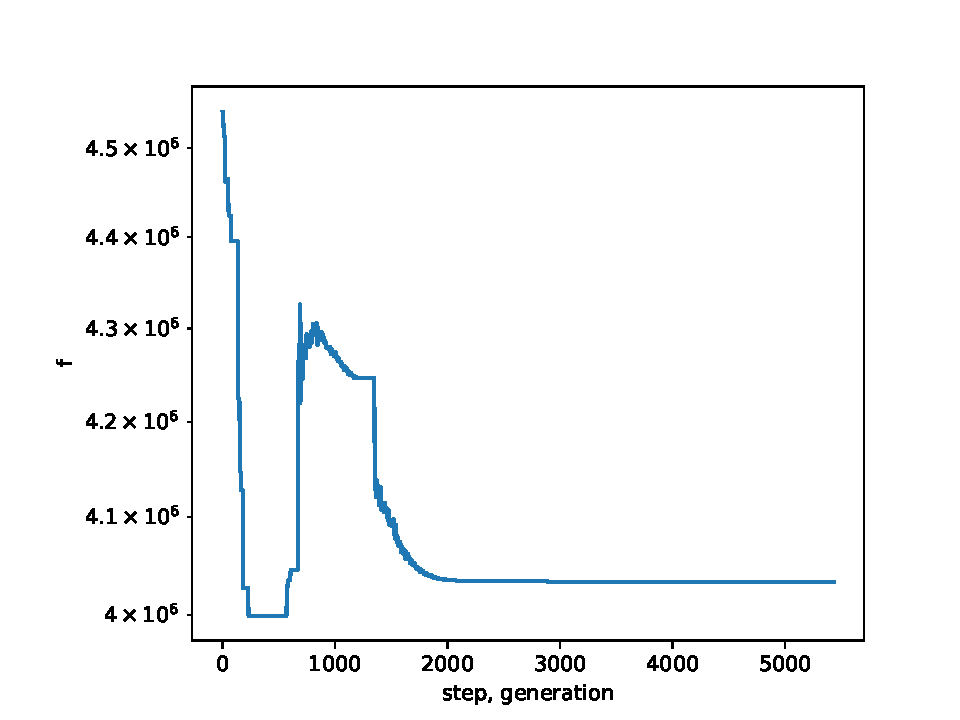
\includegraphics[width=9cm]{img_f.pdf}
        \caption{目的関数値の推移}
    \end{figure}

    \begin{figure}	%図2
        \centering
        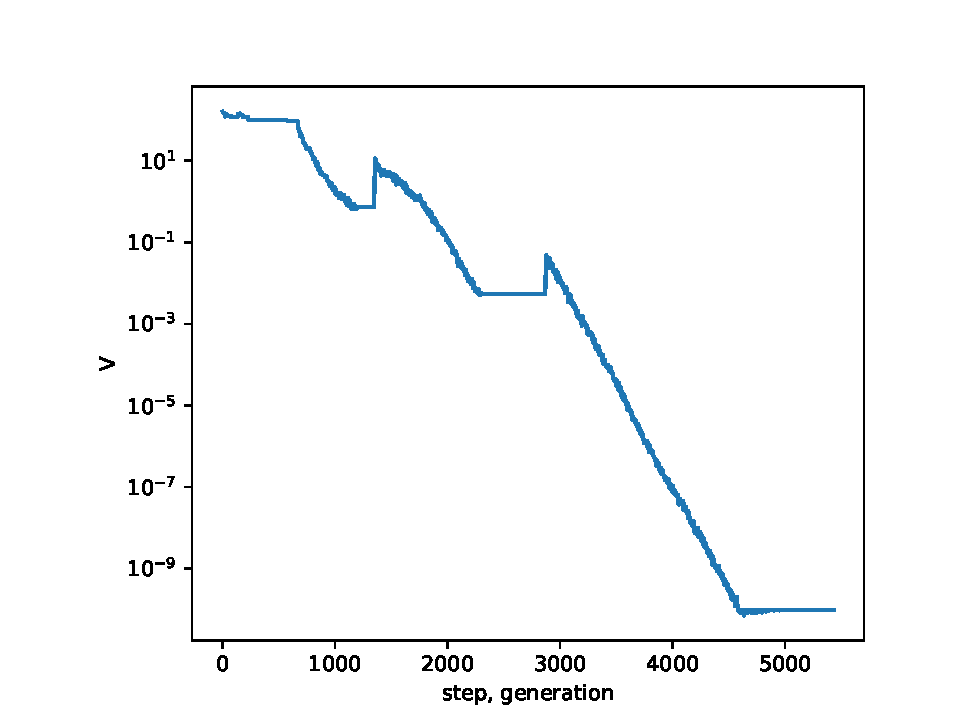
\includegraphics[width=9cm]{img_V.pdf}
        \caption{制約違反値の推移}
    \end{figure}
    結果として,実行可能解を得ることができた.ネルダーミードの探索は高速であり,およその実行可能解を探せるのではないかと考えた.また,CMA-ESにおいてペナルティ関数の係数を小さくし,目的関数が閾値より小さくなったらペナルティを与える方法は有効ではないかと考えた.


\section{今後の展望}
    一部固定ネルダーミード法とCMA-ESを組み合わせたパラメータの調整及び,数理計画ソルバーの検討をしたい.


% 参考文献
\bibliography{hoge}				%hogeはbibファイルのファイル名
\bibliographystyle{junsrt}		%順番に表示

\end{document}